\documentclass[11pt]{article}
\usepackage[top=20mm,bottom=30mm,left=20mm,right=20mm]{geometry}
\usepackage[utf8]{inputenc}
\usepackage{parskip}

% Mathy stuff
\usepackage{physics}
\usepackage{siunitx}
\usepackage{amsmath}
\usepackage[version=4]{mhchem}

% Visual stuff
\usepackage{graphics}
\usepackage{tikz}
\usetikzlibrary{math}
\usepackage{stackengine}
\usepackage{float}
\usepackage{floatpag}
\usepackage{tcolorbox}

% Misc
\usepackage{cleveref}
\usepackage{lipsum}

\allowdisplaybreaks

\setlength{\parskip}{2ex}
\setlength{\parindent}{0em}

\newcommand\set[1]{\ensuremath{\{#1\}}}
\newcommand\textbff[1]{\textbf{\boldmath #1}}
\newcommand{\shortnote}[1]{\textit{\footnotesize (#1)}}

\stackMath
\newcommand{\suf}[2]{\stackunder[0.5pt]{\stackunder[1pt]{\ensuremath{#1}}{\rule{\widthof{\ensuremath{#2}}*\real{0.9}}{.1ex}}}{}}
\newcommand{\duf}[2]{\stackunder[0.5pt]{\stackunder[0.8pt]{\stackunder[1pt]{\ensuremath{#1}}{\rule{\widthof{\ensuremath{#2}}*\real{0.9}}{.1ex}}}{\rule{\widthof{\ensuremath{#2}}*\real{0.9}}{.1ex}}}{}}
\newcommand{\su}[1]{\suf{#1}{#1}}
\newcommand{\du}[1]{\duf{#1}{#1}}
\newcommand{\ssu}[1]{\scriptsize\su{#1}\normalsize}
\newcommand{\sdu}[1]{\scriptsize\du{#1}\normalsize}

\newcommand{\pp}{\ensuremath{\partial}}

\begin{document}
\begin{center}
	\LARGE
	\textbf{Non-equilibrium, Stochastic Cellular Automata Model v1}
	\vspace{1em}
\end{center}
Considering a string of digits/letters etc. with each such string (potentially up to some symmetries) being considered a microstate of the system.
In the simplest case it seems logical to focus on models where changing any one digit is one transition.

\section{Binary Strings with Single Digits Transitions dependent on NNs}
The simplest place to start seems to be binary strings with any transition rates only dependent on (up to) its two neighbours (can be chiral).
Besides, this we ought to consider what biophysical mechanisms facilitate these transitions.
Firstly, these must be affected by the outside environment and these transitions also must affect the outside environment as otherwise by detailed balance any inverse transitions would have to be at the same rate.
This means that in a binary model, even if we had different mechanisms for each combination of neighbours, as for each of those the $0\rightarrow1$ and $1\rightarrow0$ reactions have the same rate we just get a random string.
This means that for each mechanism we will have
\begin{equation}
	\ce{\text{env} + \overline{?0?} <=>[$r_{\text{mech},f}$][$r_{\text{mech},b}$] \overline{?1?} + \text{env}^'} \qq{with} \frac{r_f}{r_b} = \exp{\beta \mu_\text{mech}}
\end{equation}
with it potentially coupling to different neighbor combinations at different rates which may be given in a matrix $K_\text{mech}$ such that the reaction rates for
\begin{equation}
	\ce{\text{env} + \overline{i0j} <=>[$r_{\text{mech},ij,f}$][$r_{\text{mech},ij,b}$] \overline{i1j} + \text{env}^'}
\end{equation}
are given by
\begin{align}
	 & r_{\text{mech},ij,f} = K_{\text{mech},ij} \frac{\exp(\beta\mu_\text{mech})}{\exp(\beta\mu_\text{mech})+1} \label{eq:rfmech} \\
	 & r_{\text{mech},ij,b} = K_{\text{mech},ij} \frac{1}{\exp(\beta\mu_\text{mech})+1} \label{eq:rbmech}
\end{align}
in the future different shorthand notations may be used.
Also note that in this binary model any forward rate always corresponds to a $0\rightarrow1$ reaction and vice-versa.
\begin{tcolorbox}
	So in summary each mechanism has its $\mu$ (originating either from energetics or effects on the outside environment) which sets the balance of 0 to 1 and 1 to 0 rates.
	And a $K$ which sets the overall rates depending on neighbours of the affected digit.
	The total rate of a particular transition is then a sum over all the mechanisms rates which are given by \cref{eq:rfmech,eq:rbmech}.
    Also, worth noting is the case of a mechanism being maximally driven, this results in that given mechanism only facilitating 0 to 1 or 1 to 0 transitions and is perhaps the most intuitive unit to start looking at.
\end{tcolorbox}

\subsection{Symmetries and $K$}
Firstly, to reduce the number of different setups we have to consider examine the symmetries which in particular affect $K$.
The only one that is always present is exchanging all 0s and 1s.
For any $K$ this comes down to a point reflection around the middle of the matrix.
Thus, if any two configurations have all $K$s such that they are such reflections of each other than those systems will have the same behaviours just with all their respective microstates being related by exchanging all 0s and 1s.

More conceptually complex is left right reflection.
The way the setup is currently described it is worth noting that the digit strings are implicitly oriented, meaning we do not consider $10011$ and $11001$ to be the same string.
This is the simplest way of working and does allow for chiral systems, in a biological sense this corresponds to something along the lines of squares and circles being placed on an explicitly oriented arrow.
The corresponding transformation of the $K$s is to take their transpose, so similarly to before two systems where all $K$s are transposes of each other will have the "same" behaviour.

Another, optional symmetry of sorts is worth noting and that is offsets and whether we consider the string to be looped or a chain with boundaries.
We mostly look at loop geometries meaning we consider the leftmost digit to be the right neighbour of the rightmost digit and vice-versa.
That said, we do not reduce the microstates, as in we do consider $0001$ and $0010$ to be different microstates, they just will have the same sort of interactions.
I do believe this is the correct way of doing things here as it accounts for the entropic factors of the biophysical microstates.
I am not quite sure at this point what the best way is to deal with chain geometries, but could involve more parameters.

The left right symmetry is worth addressing in more detail.
If we wanted to work on squares and circles on an unoriented line instead then I think one valid way of adjusting the $K$s correctly is to do $K_{ij} \rightarrow K_{ij} + (1-\delta_{ij})K_{ji}$ (no einsum) which corresponds to allowing the hypothetical enzyme to flip itself and still work.
Alternatively, one can just consider all the hypothetical enzymes to not know about this direction which is just equivalent to choosing only symmetric $K$s.
Ultimately which of these is appropriate depends on if there are really 2 enzymes one for each direction and the string loses its direction, or is there only one enzyme which just cannot tell read the direction of the string.


\subsection{Single mechanism}
Notably, this cannot give rise to an out-of-equilibrium system, but it is still worth exploring.
This gives us a single $\mu$ and $K$, leaving $\mu$ be for a bit, what options do we have for $K$.
If we at first only allow $K_{ij}\in\{0,1\}$ we have $2^4$ options however many show the same behaviour due to the symmetries described above.
All the others are enumerated in \cref{tab:KsN31M}.
Note that all of the arrows here are double-headed, that said that is assuming finite $\mu$.
$\mu$ essentially biases a mechanism towards turning 0s to 1s or otherwise, if it is 1 0 then it is unbiased but taking limits to $\pm \inf$ can make a mechanism affect only one direction.

\begin{table}
	\centering
	\tikzmath{
		\cubea = 1.5;
		\cornerR = 0.03;
	}
	\begin{tabular}{ c | c | c | c | c }
		$K$                                    & transitions                                                                                        & degen., sym.                 & Elementary trans. & All $N=3$ trans. \\
		\hline
		$\begin{pmatrix}0&0\\0&0\end{pmatrix}$ & \begin{minipage}{0.1\textwidth} none \end{minipage}                                                & 1, none                      &
		\begin{minipage}{0.2\textwidth}
			\centering
			\vspace{0.3em}
			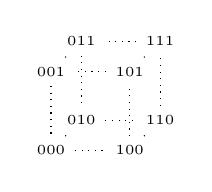
\begin{tikzpicture}
				\node (X000) at (0,0,\cubea) {\tiny 000};
				\node (X100) at (\cubea,0,\cubea) {\tiny 100};
				\node (X010) at (0,0,0) {\tiny 010};
				\node (X001) at (0,\cubea,\cubea) {\tiny 001};
				\node (X011) at (0,\cubea,0) {\tiny 011};
				\node (X101) at (\cubea,\cubea,\cubea) {\tiny 101};
				\node (X110) at (\cubea,0,0) {\tiny 110};
				\node (X111) at (\cubea,\cubea,0) {\tiny 111};

				% front face
				\draw[dotted] (X000) -- (X100);
				\draw[dotted] (X100) -- (X101);
				\draw[dotted] (X101) -- (X001);
				\draw[dotted] (X001) -- (X000);
				% back face
				\draw[dotted] (X010) -- (X110);
				\draw[dotted] (X110) -- (X111);
				\draw[dotted] (X111) -- (X011);
				\draw[dotted] (X011) -- (X010);
				% the lines connecting them
				\draw[dotted] (X000) -- (X010);
				\draw[dotted] (X100) -- (X110);
				\draw[dotted] (X101) -- (X111);
				\draw[dotted] (X001) -- (X011);
			\end{tikzpicture}
			\vspace{0.3em}
		\end{minipage}        & \begin{minipage}{0.2\textwidth}
			                        \centering
			                        \vspace{0.3em}
			                        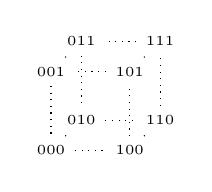
\begin{tikzpicture}
				\node (X000) at (0,0,\cubea) {\tiny 000};
				\node (X100) at (\cubea,0,\cubea) {\tiny 100};
				\node (X010) at (0,0,0) {\tiny 010};
				\node (X001) at (0,\cubea,\cubea) {\tiny 001};
				\node (X011) at (0,\cubea,0) {\tiny 011};
				\node (X101) at (\cubea,\cubea,\cubea) {\tiny 101};
				\node (X110) at (\cubea,0,0) {\tiny 110};
				\node (X111) at (\cubea,\cubea,0) {\tiny 111};

				% front face
				\draw[dotted] (X000) -- (X100);
				\draw[dotted] (X100) -- (X101);
				\draw[dotted] (X101) -- (X001);
				\draw[dotted] (X001) -- (X000);
				% back face
				\draw[dotted] (X010) -- (X110);
				\draw[dotted] (X110) -- (X111);
				\draw[dotted] (X111) -- (X011);
				\draw[dotted] (X011) -- (X010);
				% the lines connecting them
				\draw[dotted] (X000) -- (X010);
				\draw[dotted] (X100) -- (X110);
				\draw[dotted] (X101) -- (X111);
				\draw[dotted] (X001) -- (X011);
			\end{tikzpicture}
			                        \vspace{0.3em}
		                        \end{minipage}                                                                                                                                                            \\
		\hline
		$\begin{pmatrix}1&0\\0&0\end{pmatrix}$ & \begin{minipage}{0.1\textwidth} $000 \leftrightarrow 010$ \end{minipage}                           & 2, via $0 \leftrightarrow 1$ &
		\begin{minipage}{0.2\textwidth}
			\centering
			\vspace{0.3em}
			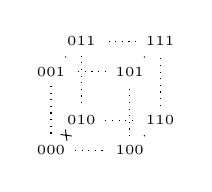
\begin{tikzpicture}
				\node (X000) at (0,0,\cubea) {\tiny 000};
				\node (X100) at (\cubea,0,\cubea) {\tiny 100};
				\node (X010) at (0,0,0) {\tiny 010};
				\node (X001) at (0,\cubea,\cubea) {\tiny 001};
				\node (X011) at (0,\cubea,0) {\tiny 011};
				\node (X101) at (\cubea,\cubea,\cubea) {\tiny 101};
				\node (X110) at (\cubea,0,0) {\tiny 110};
				\node (X111) at (\cubea,\cubea,0) {\tiny 111};

				% front face
				\draw[dotted] (X000) -- (X100);
				\draw[dotted] (X100) -- (X101);
				\draw[dotted] (X101) -- (X001);
				\draw[dotted] (X001) -- (X000);
				% back face
				\draw[dotted] (X010) -- (X110);
				\draw[dotted] (X110) -- (X111);
				\draw[dotted] (X111) -- (X011);
				\draw[dotted] (X011) -- (X010);
				% the lines connecting them
				\draw[<->] (X000) -- (X010);
				\draw[dotted] (X100) -- (X110);
				\draw[dotted] (X101) -- (X111);
				\draw[dotted] (X001) -- (X011);
			\end{tikzpicture}
			\vspace{0.3em}
		\end{minipage}        & \begin{minipage}{0.2\textwidth}
			                        \centering
			                        \vspace{0.3em}
			                        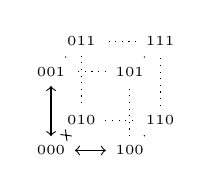
\begin{tikzpicture}
				\node (X000) at (0,0,\cubea) {\tiny 000};
				\node (X100) at (\cubea,0,\cubea) {\tiny 100};
				\node (X010) at (0,0,0) {\tiny 010};
				\node (X001) at (0,\cubea,\cubea) {\tiny 001};
				\node (X011) at (0,\cubea,0) {\tiny 011};
				\node (X101) at (\cubea,\cubea,\cubea) {\tiny 101};
				\node (X110) at (\cubea,0,0) {\tiny 110};
				\node (X111) at (\cubea,\cubea,0) {\tiny 111};

				% front face
				\draw[<->] (X000) -- (X100);
				\draw[dotted] (X100) -- (X101);
				\draw[dotted] (X101) -- (X001);
				\draw[<->] (X001) -- (X000);
				% back face
				\draw[dotted] (X010) -- (X110);
				\draw[dotted] (X110) -- (X111);
				\draw[dotted] (X111) -- (X011);
				\draw[dotted] (X011) -- (X010);
				% the lines connecting them
				\draw[<->] (X000) -- (X010);
				\draw[dotted] (X100) -- (X110);
				\draw[dotted] (X101) -- (X111);
				\draw[dotted] (X001) -- (X011);
			\end{tikzpicture}
			                        \vspace{0.3em}
		                        \end{minipage}                                                                                                                                                            \\
		\hline
		$\begin{pmatrix}0&0\\1&0\end{pmatrix}$ & \begin{minipage}{0.1\textwidth} $100 \leftrightarrow 110$ \end{minipage}                           & 2, via either                &
		\begin{minipage}{0.2\textwidth}
			\centering
			\vspace{0.3em}
			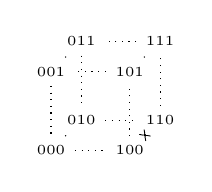
\begin{tikzpicture}
				\node (X000) at (0,0,\cubea) {\tiny 000};
				\node (X100) at (\cubea,0,\cubea) {\tiny 100};
				\node (X010) at (0,0,0) {\tiny 010};
				\node (X001) at (0,\cubea,\cubea) {\tiny 001};
				\node (X011) at (0,\cubea,0) {\tiny 011};
				\node (X101) at (\cubea,\cubea,\cubea) {\tiny 101};
				\node (X110) at (\cubea,0,0) {\tiny 110};
				\node (X111) at (\cubea,\cubea,0) {\tiny 111};

				% front face
				\draw[dotted] (X000) -- (X100);
				\draw[dotted] (X100) -- (X101);
				\draw[dotted] (X101) -- (X001);
				\draw[dotted] (X001) -- (X000);
				% back face
				\draw[dotted] (X010) -- (X110);
				\draw[dotted] (X110) -- (X111);
				\draw[dotted] (X111) -- (X011);
				\draw[dotted] (X011) -- (X010);
				% the lines connecting them
				\draw[dotted] (X000) -- (X010);
				\draw[<->] (X100) -- (X110);
				\draw[dotted] (X101) -- (X111);
				\draw[dotted] (X001) -- (X011);
			\end{tikzpicture}
			\vspace{0.3em}
		\end{minipage}        & \begin{minipage}{0.2\textwidth}
			                        \centering
			                        \vspace{0.3em}
			                        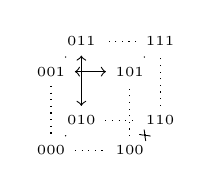
\begin{tikzpicture}
				\node (X000) at (0,0,\cubea) {\tiny 000};
				\node (X100) at (\cubea,0,\cubea) {\tiny 100};
				\node (X010) at (0,0,0) {\tiny 010};
				\node (X001) at (0,\cubea,\cubea) {\tiny 001};
				\node (X011) at (0,\cubea,0) {\tiny 011};
				\node (X101) at (\cubea,\cubea,\cubea) {\tiny 101};
				\node (X110) at (\cubea,0,0) {\tiny 110};
				\node (X111) at (\cubea,\cubea,0) {\tiny 111};

				% front face
				\draw[dotted] (X000) -- (X100);
				\draw[dotted] (X100) -- (X101);
				\draw[<->] (X101) -- (X001);
				\draw[dotted] (X001) -- (X000);
				% back face
				\draw[dotted] (X010) -- (X110);
				\draw[dotted] (X110) -- (X111);
				\draw[dotted] (X111) -- (X011);
				\draw[<->] (X011) -- (X010);
				% the lines connecting them
				\draw[dotted] (X000) -- (X010);
				\draw[<->] (X100) -- (X110);
				\draw[dotted] (X101) -- (X111);
				\draw[dotted] (X001) -- (X011);
			\end{tikzpicture}
			                        \vspace{0.3em}
		                        \end{minipage}                                                                                                                                                            \\
		\hline
		$\begin{pmatrix}1&0\\0&1\end{pmatrix}$ & \begin{minipage}{0.1\textwidth} $000 \leftrightarrow 010$ $101 \leftrightarrow 111$ \end{minipage} & 1, none                      &
		\begin{minipage}{0.2\textwidth}
			\centering
			\vspace{0.3em}
			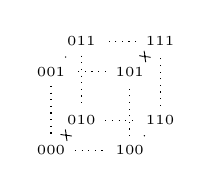
\begin{tikzpicture}
				\node (X000) at (0,0,\cubea) {\tiny 000};
				\node (X100) at (\cubea,0,\cubea) {\tiny 100};
				\node (X010) at (0,0,0) {\tiny 010};
				\node (X001) at (0,\cubea,\cubea) {\tiny 001};
				\node (X011) at (0,\cubea,0) {\tiny 011};
				\node (X101) at (\cubea,\cubea,\cubea) {\tiny 101};
				\node (X110) at (\cubea,0,0) {\tiny 110};
				\node (X111) at (\cubea,\cubea,0) {\tiny 111};

				% front face
				\draw[dotted] (X000) -- (X100);
				\draw[dotted] (X100) -- (X101);
				\draw[dotted] (X101) -- (X001);
				\draw[dotted] (X001) -- (X000);
				% back face
				\draw[dotted] (X010) -- (X110);
				\draw[dotted] (X110) -- (X111);
				\draw[dotted] (X111) -- (X011);
				\draw[dotted] (X011) -- (X010);
				% the lines connecting them
				\draw[<->] (X000) -- (X010);
				\draw[dotted] (X100) -- (X110);
				\draw[<->] (X101) -- (X111);
				\draw[dotted] (X001) -- (X011);
			\end{tikzpicture}
			\vspace{0.3em}
		\end{minipage}        & \begin{minipage}{0.2\textwidth}
			                        \centering
			                        \vspace{0.3em}
			                        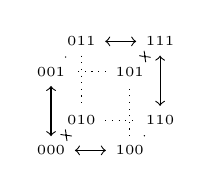
\begin{tikzpicture}
				\node (X000) at (0,0,\cubea) {\tiny 000};
				\node (X100) at (\cubea,0,\cubea) {\tiny 100};
				\node (X010) at (0,0,0) {\tiny 010};
				\node (X001) at (0,\cubea,\cubea) {\tiny 001};
				\node (X011) at (0,\cubea,0) {\tiny 011};
				\node (X101) at (\cubea,\cubea,\cubea) {\tiny 101};
				\node (X110) at (\cubea,0,0) {\tiny 110};
				\node (X111) at (\cubea,\cubea,0) {\tiny 111};

				% front face
				\draw[<->] (X000) -- (X100);
				\draw[dotted] (X100) -- (X101);
				\draw[dotted] (X101) -- (X001);
				\draw[<->] (X001) -- (X000);
				% back face
				\draw[dotted] (X010) -- (X110);
				\draw[<->] (X110) -- (X111);
				\draw[<->] (X111) -- (X011);
				\draw[dotted] (X011) -- (X010);
				% the lines connecting them
				\draw[<->] (X000) -- (X010);
				\draw[dotted] (X100) -- (X110);
				\draw[<->] (X101) -- (X111);
				\draw[dotted] (X001) -- (X011);
			\end{tikzpicture}
			                        \vspace{0.3em}
		                        \end{minipage}                                                                                                                                                            \\
		\hline
		$\begin{pmatrix}0&1\\1&0\end{pmatrix}$ & \begin{minipage}{0.1\textwidth} $001 \leftrightarrow 011$ $100 \leftrightarrow 110$ \end{minipage} & 1, none                      &
		\begin{minipage}{0.2\textwidth}
			\centering
			\vspace{0.3em}
			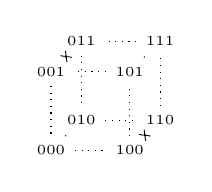
\begin{tikzpicture}
				\node (X000) at (0,0,\cubea) {\tiny 000};
				\node (X100) at (\cubea,0,\cubea) {\tiny 100};
				\node (X010) at (0,0,0) {\tiny 010};
				\node (X001) at (0,\cubea,\cubea) {\tiny 001};
				\node (X011) at (0,\cubea,0) {\tiny 011};
				\node (X101) at (\cubea,\cubea,\cubea) {\tiny 101};
				\node (X110) at (\cubea,0,0) {\tiny 110};
				\node (X111) at (\cubea,\cubea,0) {\tiny 111};

				% front face
				\draw[dotted] (X000) -- (X100);
				\draw[dotted] (X100) -- (X101);
				\draw[dotted] (X101) -- (X001);
				\draw[dotted] (X001) -- (X000);
				% back face
				\draw[dotted] (X010) -- (X110);
				\draw[dotted] (X110) -- (X111);
				\draw[dotted] (X111) -- (X011);
				\draw[dotted] (X011) -- (X010);
				% the lines connecting them
				\draw[dotted] (X000) -- (X010);
				\draw[<->] (X100) -- (X110);
				\draw[dotted] (X101) -- (X111);
				\draw[<->] (X001) -- (X011);
			\end{tikzpicture}
			\vspace{0.3em}
		\end{minipage}        & \begin{minipage}{0.2\textwidth}
			                        \centering
			                        \vspace{0.3em}
			                        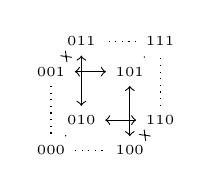
\begin{tikzpicture}
				\node (X000) at (0,0,\cubea) {\tiny 000};
				\node (X100) at (\cubea,0,\cubea) {\tiny 100};
				\node (X010) at (0,0,0) {\tiny 010};
				\node (X001) at (0,\cubea,\cubea) {\tiny 001};
				\node (X011) at (0,\cubea,0) {\tiny 011};
				\node (X101) at (\cubea,\cubea,\cubea) {\tiny 101};
				\node (X110) at (\cubea,0,0) {\tiny 110};
				\node (X111) at (\cubea,\cubea,0) {\tiny 111};

				% front face
				\draw[dotted] (X000) -- (X100);
				\draw[<->] (X100) -- (X101);
				\draw[<->] (X101) -- (X001);
				\draw[dotted] (X001) -- (X000);
				% back face
				\draw[<->] (X010) -- (X110);
				\draw[dotted] (X110) -- (X111);
				\draw[dotted] (X111) -- (X011);
				\draw[<->] (X011) -- (X010);
				% the lines connecting them
				\draw[dotted] (X000) -- (X010);
				\draw[<->] (X100) -- (X110);
				\draw[dotted] (X101) -- (X111);
				\draw[<->] (X001) -- (X011);
			\end{tikzpicture}
			                        \vspace{0.3em}
		                        \end{minipage}                                                                                                                                                            \\
		\hline
		$\begin{pmatrix}1&0\\1&0\end{pmatrix}$ & \begin{minipage}{0.1\textwidth} $000 \leftrightarrow 010$ $100 \leftrightarrow 110$ \end{minipage} & 4, via combinations of both  &
		\begin{minipage}{0.2\textwidth}
			\centering
			\vspace{0.3em}
			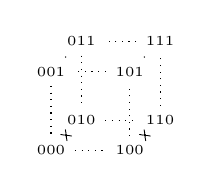
\begin{tikzpicture}
				\node (X000) at (0,0,\cubea) {\tiny 000};
				\node (X100) at (\cubea,0,\cubea) {\tiny 100};
				\node (X010) at (0,0,0) {\tiny 010};
				\node (X001) at (0,\cubea,\cubea) {\tiny 001};
				\node (X011) at (0,\cubea,0) {\tiny 011};
				\node (X101) at (\cubea,\cubea,\cubea) {\tiny 101};
				\node (X110) at (\cubea,0,0) {\tiny 110};
				\node (X111) at (\cubea,\cubea,0) {\tiny 111};

				% front face
				\draw[dotted] (X000) -- (X100);
				\draw[dotted] (X100) -- (X101);
				\draw[dotted] (X101) -- (X001);
				\draw[dotted] (X001) -- (X000);
				% back face
				\draw[dotted] (X010) -- (X110);
				\draw[dotted] (X110) -- (X111);
				\draw[dotted] (X111) -- (X011);
				\draw[dotted] (X011) -- (X010);
				% the lines connecting them
				\draw[<->] (X000) -- (X010);
				\draw[<->] (X100) -- (X110);
				\draw[dotted] (X101) -- (X111);
				\draw[dotted] (X001) -- (X011);
			\end{tikzpicture}
			\vspace{0.3em}
		\end{minipage}        & \begin{minipage}{0.2\textwidth}
			                        \centering
			                        \vspace{0.3em}
			                        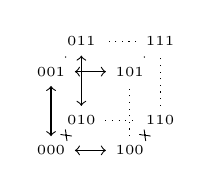
\begin{tikzpicture}
				\node (X000) at (0,0,\cubea) {\tiny 000};
				\node (X100) at (\cubea,0,\cubea) {\tiny 100};
				\node (X010) at (0,0,0) {\tiny 010};
				\node (X001) at (0,\cubea,\cubea) {\tiny 001};
				\node (X011) at (0,\cubea,0) {\tiny 011};
				\node (X101) at (\cubea,\cubea,\cubea) {\tiny 101};
				\node (X110) at (\cubea,0,0) {\tiny 110};
				\node (X111) at (\cubea,\cubea,0) {\tiny 111};

				% front face
				\draw[<->] (X000) -- (X100);
				\draw[dotted] (X100) -- (X101);
				\draw[<->] (X101) -- (X001);
				\draw[<->] (X001) -- (X000);
				% back face
				\draw[dotted] (X010) -- (X110);
				\draw[dotted] (X110) -- (X111);
				\draw[dotted] (X111) -- (X011);
				\draw[<->] (X011) -- (X010);
				% the lines connecting them
				\draw[<->] (X000) -- (X010);
				\draw[<->] (X100) -- (X110);
				\draw[dotted] (X101) -- (X111);
				\draw[dotted] (X001) -- (X011);
			\end{tikzpicture}
			                        \vspace{0.3em}
		                        \end{minipage}                                                                                                                                                            \\
		\hline
		$\begin{pmatrix}1&1\\1&0\end{pmatrix}$ & \begin{minipage}{0.1\textwidth} all except $101 \leftrightarrow 111$ \end{minipage}                & 2, via $0 \leftrightarrow 1$ &
		\begin{minipage}{0.2\textwidth}
			\centering
			\vspace{0.3em}
			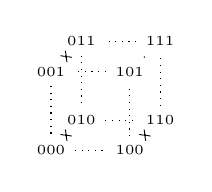
\begin{tikzpicture}
				\node (X000) at (0,0,\cubea) {\tiny 000};
				\node (X100) at (\cubea,0,\cubea) {\tiny 100};
				\node (X010) at (0,0,0) {\tiny 010};
				\node (X001) at (0,\cubea,\cubea) {\tiny 001};
				\node (X011) at (0,\cubea,0) {\tiny 011};
				\node (X101) at (\cubea,\cubea,\cubea) {\tiny 101};
				\node (X110) at (\cubea,0,0) {\tiny 110};
				\node (X111) at (\cubea,\cubea,0) {\tiny 111};

				% front face
				\draw[dotted] (X000) -- (X100);
				\draw[dotted] (X100) -- (X101);
				\draw[dotted] (X101) -- (X001);
				\draw[dotted] (X001) -- (X000);
				% back face
				\draw[dotted] (X010) -- (X110);
				\draw[dotted] (X110) -- (X111);
				\draw[dotted] (X111) -- (X011);
				\draw[dotted] (X011) -- (X010);
				% the lines connecting them
				\draw[<->] (X000) -- (X010);
				\draw[<->] (X100) -- (X110);
				\draw[dotted] (X101) -- (X111);
				\draw[<->] (X001) -- (X011);
			\end{tikzpicture}
			\vspace{0.3em}
		\end{minipage}        & \begin{minipage}{0.2\textwidth}
			                        \centering
			                        \vspace{0.3em}
			                        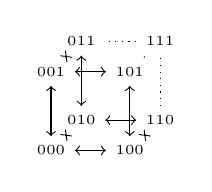
\begin{tikzpicture}
				\node (X000) at (0,0,\cubea) {\tiny 000};
				\node (X100) at (\cubea,0,\cubea) {\tiny 100};
				\node (X010) at (0,0,0) {\tiny 010};
				\node (X001) at (0,\cubea,\cubea) {\tiny 001};
				\node (X011) at (0,\cubea,0) {\tiny 011};
				\node (X101) at (\cubea,\cubea,\cubea) {\tiny 101};
				\node (X110) at (\cubea,0,0) {\tiny 110};
				\node (X111) at (\cubea,\cubea,0) {\tiny 111};

				% front face
				\draw[<->] (X000) -- (X100);
				\draw[<->] (X100) -- (X101);
				\draw[<->] (X101) -- (X001);
				\draw[<->] (X001) -- (X000);
				% back face
				\draw[<->] (X010) -- (X110);
				\draw[dotted] (X110) -- (X111);
				\draw[dotted] (X111) -- (X011);
				\draw[<->] (X011) -- (X010);
				% the lines connecting them
				\draw[<->] (X000) -- (X010);
				\draw[<->] (X100) -- (X110);
				\draw[dotted] (X101) -- (X111);
				\draw[<->] (X001) -- (X011);
			\end{tikzpicture}
			                        \vspace{0.3em}
		                        \end{minipage}                                                                                                                                                            \\
		\hline
		$\begin{pmatrix}1&1\\0&1\end{pmatrix}$ & \begin{minipage}{0.1\textwidth} all except $100 \leftrightarrow 110$ \end{minipage}                & 2, via either                &
		\begin{minipage}{0.2\textwidth}
			\centering
			\vspace{0.3em}
			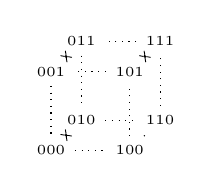
\begin{tikzpicture}
				\node (X000) at (0,0,\cubea) {\tiny 000};
				\node (X100) at (\cubea,0,\cubea) {\tiny 100};
				\node (X010) at (0,0,0) {\tiny 010};
				\node (X001) at (0,\cubea,\cubea) {\tiny 001};
				\node (X011) at (0,\cubea,0) {\tiny 011};
				\node (X101) at (\cubea,\cubea,\cubea) {\tiny 101};
				\node (X110) at (\cubea,0,0) {\tiny 110};
				\node (X111) at (\cubea,\cubea,0) {\tiny 111};

				% front face
				\draw[dotted] (X000) -- (X100);
				\draw[dotted] (X100) -- (X101);
				\draw[dotted] (X101) -- (X001);
				\draw[dotted] (X001) -- (X000);
				% back face
				\draw[dotted] (X010) -- (X110);
				\draw[dotted] (X110) -- (X111);
				\draw[dotted] (X111) -- (X011);
				\draw[dotted] (X011) -- (X010);
				% the lines connecting them
				\draw[<->] (X000) -- (X010);
				\draw[dotted] (X100) -- (X110);
				\draw[<->] (X101) -- (X111);
				\draw[<->] (X001) -- (X011);
			\end{tikzpicture}
			\vspace{0.3em}
		\end{minipage}        & \begin{minipage}{0.2\textwidth}
			                        \centering
			                        \vspace{0.3em}
			                        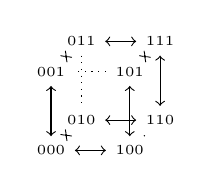
\begin{tikzpicture}
				\node (X000) at (0,0,\cubea) {\tiny 000};
				\node (X100) at (\cubea,0,\cubea) {\tiny 100};
				\node (X010) at (0,0,0) {\tiny 010};
				\node (X001) at (0,\cubea,\cubea) {\tiny 001};
				\node (X011) at (0,\cubea,0) {\tiny 011};
				\node (X101) at (\cubea,\cubea,\cubea) {\tiny 101};
				\node (X110) at (\cubea,0,0) {\tiny 110};
				\node (X111) at (\cubea,\cubea,0) {\tiny 111};

				% front face
				\draw[<->] (X000) -- (X100);
				\draw[<->] (X100) -- (X101);
				\draw[dotted] (X101) -- (X001);
				\draw[<->] (X001) -- (X000);
				% back face
				\draw[<->] (X010) -- (X110);
				\draw[<->] (X110) -- (X111);
				\draw[<->] (X111) -- (X011);
				\draw[dotted] (X011) -- (X010);
				% the lines connecting them
				\draw[<->] (X000) -- (X010);
				\draw[dotted] (X100) -- (X110);
				\draw[<->] (X101) -- (X111);
				\draw[<->] (X001) -- (X011);
			\end{tikzpicture}
			                        \vspace{0.3em}
		                        \end{minipage}                                                                                                                                                            \\
		\hline
		$\begin{pmatrix}1&1\\1&1\end{pmatrix}$ & \begin{minipage}{0.1\textwidth} all \end{minipage}                                                 & 1, none                      &
		\begin{minipage}{0.2\textwidth}
			\centering
			\vspace{0.3em}
			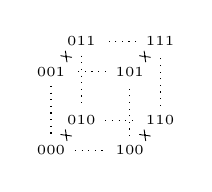
\begin{tikzpicture}
				\node (X000) at (0,0,\cubea) {\tiny 000};
				\node (X100) at (\cubea,0,\cubea) {\tiny 100};
				\node (X010) at (0,0,0) {\tiny 010};
				\node (X001) at (0,\cubea,\cubea) {\tiny 001};
				\node (X011) at (0,\cubea,0) {\tiny 011};
				\node (X101) at (\cubea,\cubea,\cubea) {\tiny 101};
				\node (X110) at (\cubea,0,0) {\tiny 110};
				\node (X111) at (\cubea,\cubea,0) {\tiny 111};

				% front face
				\draw[dotted] (X000) -- (X100);
				\draw[dotted] (X100) -- (X101);
				\draw[dotted] (X101) -- (X001);
				\draw[dotted] (X001) -- (X000);
				% back face
				\draw[dotted] (X010) -- (X110);
				\draw[dotted] (X110) -- (X111);
				\draw[dotted] (X111) -- (X011);
				\draw[dotted] (X011) -- (X010);
				% the lines connecting them
				\draw[<->] (X000) -- (X010);
				\draw[<->] (X100) -- (X110);
				\draw[<->] (X101) -- (X111);
				\draw[<->] (X001) -- (X011);
			\end{tikzpicture}
			\vspace{0.3em}
		\end{minipage}        & \begin{minipage}{0.2\textwidth}
			                        \centering
			                        \vspace{0.3em}
			                        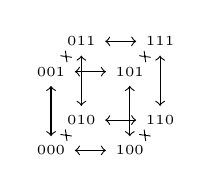
\begin{tikzpicture}
				\node (X000) at (0,0,\cubea) {\tiny 000};
				\node (X100) at (\cubea,0,\cubea) {\tiny 100};
				\node (X010) at (0,0,0) {\tiny 010};
				\node (X001) at (0,\cubea,\cubea) {\tiny 001};
				\node (X011) at (0,\cubea,0) {\tiny 011};
				\node (X101) at (\cubea,\cubea,\cubea) {\tiny 101};
				\node (X110) at (\cubea,0,0) {\tiny 110};
				\node (X111) at (\cubea,\cubea,0) {\tiny 111};

				% front face
				\draw[<->] (X000) -- (X100);
				\draw[<->] (X100) -- (X101);
				\draw[<->] (X101) -- (X001);
				\draw[<->] (X001) -- (X000);
				% back face
				\draw[<->] (X010) -- (X110);
				\draw[<->] (X110) -- (X111);
				\draw[<->] (X111) -- (X011);
				\draw[<->] (X011) -- (X010);
				% the lines connecting them
				\draw[<->] (X000) -- (X010);
				\draw[<->] (X100) -- (X110);
				\draw[<->] (X101) -- (X111);
				\draw[<->] (X001) -- (X011);
			\end{tikzpicture}
			                        \vspace{0.3em}
		                        \end{minipage}                                                                                                                                                            \\
		\hline
	\end{tabular}
	\caption{Summary of all the possible $K$s for N=3 and a single mechanism with a unique behaviour.}\label{tab:KsN31M}
\end{table}

\subsection{Two maximally driven oposing mechanisms}

\end{document}
